% !TEX root =  ../main.tex
\section{Ban}
\subsection{Definition}

\subsubsection{Signature} \cstr{ban(vs : set<VM>, ns : set<server>)}

\begin{itemize}
\item \cstr{vs} : an non-empty set of VMs for a meaningful constraint. VMs not in the \st{Running} state are ignored.
\item \cstr{ns} : an non-empty set of servers for a meaningful constraint. Servers not in the \st{Online} state are ignored.
\end{itemize}

The \cstr{ban} constraint disallows each running VM in \cstr{vs} to be hosted on any of
the online servers in \cstr{ns}.

\classification{ban}{datacenter administrator}{VM placement}{Maintenance,Partitioning,VM-to-server placement}

\subsubsection{Usage}

This constraint may be use by the datacenter administrator to prepare servers for a software maintenance.
In this situation, the administrator must first be sure that the servers do not host any running VMs to prevent a
misconfiguration from altering them. Every running VM on these servers must then be relocated elsewhere
while the other VMs should not be relocated on the servers to put into maintenance.
%
A datacenter administrator may rely on a \cstr{ban} constraint to achieve that purpose. In this setting, all
the VMs in the datacenter are given in parameters in addition to the servers to put into maintenance. At the end
of the reconfiguration, no VMs will be running on the servers.  Once the maintenance operation is terminated,
the constraint may be removed to put the servers back into the hosting pool.

For partitioning reasons, some VMs may be disallowed to be running on some servers.  As an example, servers may be dedicated to run service VMs. In this setting, the client VMs must not be allowed to run on the servers dedicated to run service VMs. \cstr{Ban} constraints may then be used by the datacenter administrator for that purpose.


\subsubsection{Example}

Figure~\ref{lst: ban} depicts a sample reconfiguration between a source and a destination configuration.
In this example, the following \cstr{ban} constraints were considered:

\begin{reconfiguration}[htb]
\centering
\begin{minipage}[b]{0.40\textwidth}
\begin{lstlisting}
N1: VM1 VM2
N2: VM4 VM3
N3: 
\end{lstlisting}
\end{minipage}
\begin{minipage}[b]{2cm}
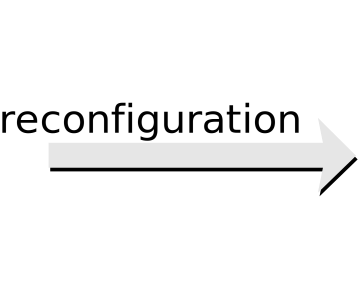
\includegraphics[width=2cm]{img/arrow_reconfiguration}
\end{minipage}
\begin{minipage}[b]{0.40\textwidth}
\begin{lstlisting}
N1: VM1
N2: (VM3)
N3: VM2 VM4
\end{lstlisting}
\end{minipage}
\caption{A reconfiguration motivated by \cstr{ban} constraints.}\label{lst: ban}
\end{reconfiguration}

\begin{itemize}
\item \cstr{ban(\{VM1, VM2, VM4\}, \{N2\})}. This constraint was not satisfied in the source configuration
as \cstr{VM4} was running on \cstr{N2}. The reconfiguration fixed this violation
by relocating \cstr{VM4} to \cstr{N3}.

\item \cstr{ban(\{VM3\}, \{N2\})}. This constraint was not satisfied in the source configuration. However it is satisfied in the destination configuration as \cstr{VM3} is no longer running.

\item \cstr{ban(\{VM1, VM2\}, \{N2\})}. This constraint was satisfied in the source configuration. It is still satisfied in the destination configuration as the relocation of \cstr{VM2} is compatible with this constraint.
\end{itemize}

\fullVersion{
\subsection{Model}

The \cstr{ban} constraint is modeled using a domain restriction on the d-slice associated to each of the running VMs.

\begin{equation*}
\begin{split}
\text{\cstr{ban(V : set<VM>, N : set<server>)}} &\triangleq\\
   & \forall v_i \in V, d_i^h \ni \{\forall j | n_j \in N\}
\end{split}
\end{equation*}

\subsection{Violation Detection}

The detection of the violating elements in \cstr{ban} consists in identifying the VMs that are hosted
on forbidden servers. The computed selection of misplaced VMs is guarantee to be minimal with regards to the scope of the constraint.

\subsection{Availability}

\subsubsection{In {\btrp}}

This constraint is available in {\btrp} using the name \texttt{ban}.
Using the Choco API, the assignment of the d-slice placement variable is pruned to remove the disallowed servers using a \emph{notMember} constraint (referred as \emph{not\_in} in the Global Constraints Catalog~\cite{gccat}).

\begin{equation*}
\begin{split}
\text{\cstr{ban(V : set<VM>, N : set<server>)}} &\triangleq\\
   & \forall v_i \in V, not\_in(d_i^h, \{\forall j | n_j \in N \})
\end{split}
\end{equation*}

\subsubsection{In VMWare}
}

\subsection{See also}

\subsubsection{Related Constraints}

\begin{itemize}
\item \cstrref{fence}: the opposite constraint of \cstr{ban}. One \cstr{ban} constraint can be emulated using a \cstr{fence} constraint by specifying to the \cstr{fence} constraint, the absolute complement of the set of servers specified in the \cstr{ban} constraint.

\item \cstrref{quarantine}. The \cstr{quarantine} constraint may also be used to prepare a software maintenance on servers when relocation is not possible. In this setting, the given servers will be ready for the maintenance once their VMs are terminated.
\end{itemize}

\emulatedWith{ban}{fence}{\cstr{ban(vs1, ns1)}}{\cstr{fence(vs1,\oline{ns1})}}
\emulatedWith{ban}{among}{\cstr{ban(vs1, ns1)}}{\cstr{among(vs1,\{\oline{ns1}\})}}
\printListOfInheritance{ban}